\documentclass{standalone}
\usepackage{tikz}
\usetikzlibrary{patterns, positioning}

\begin{document}
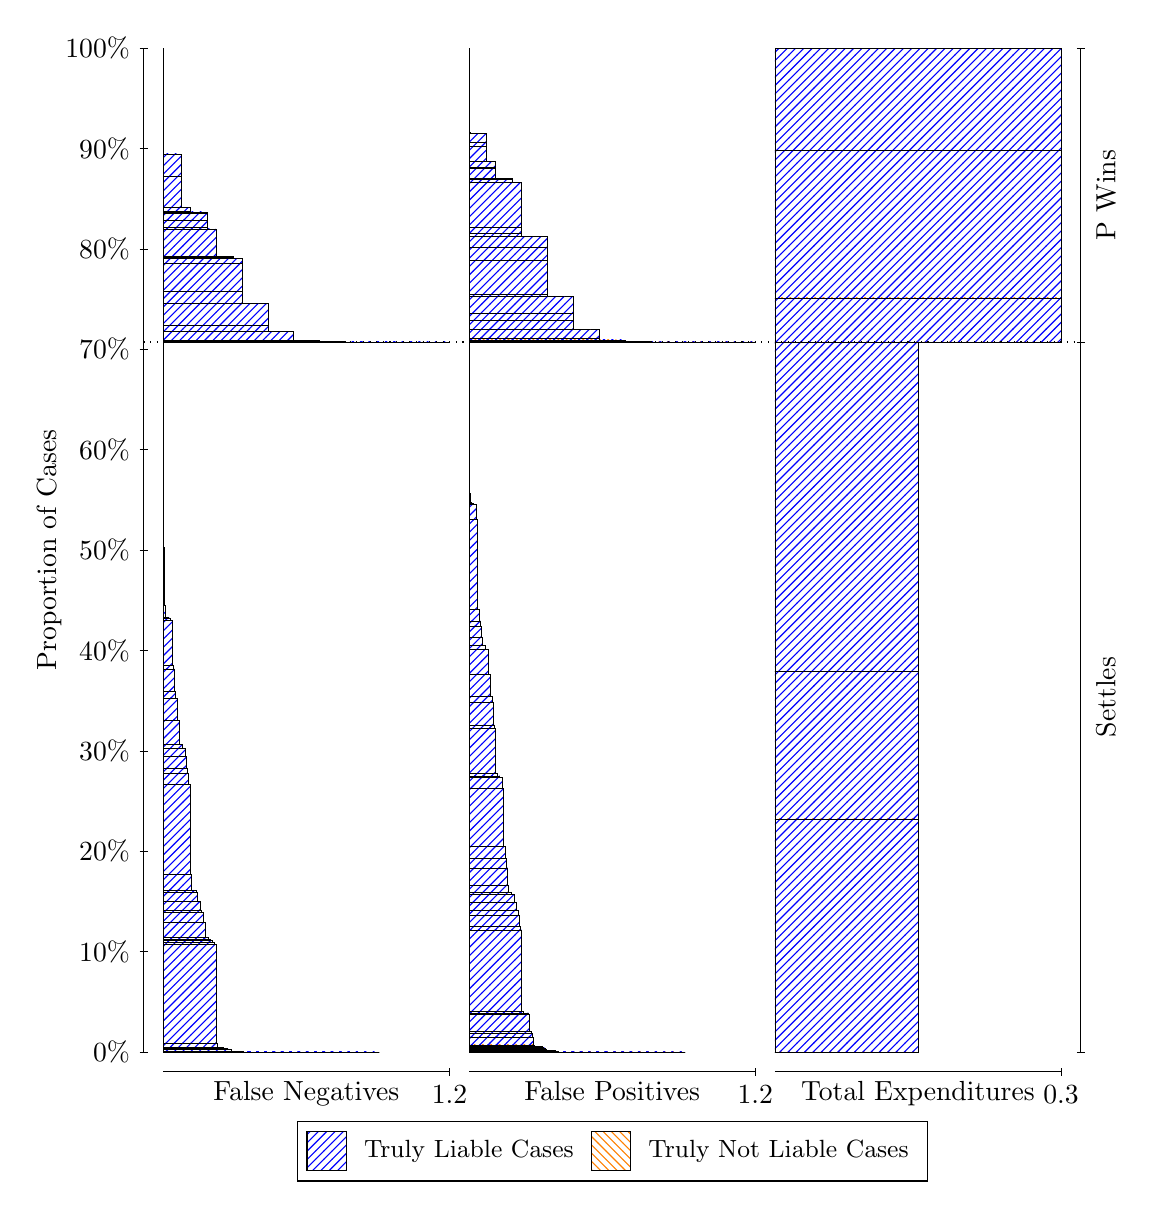
\begin{tikzpicture}
\draw[black, very thin] (1.5,1.75) -- (1.5,14.5);
\node[rotate=90, anchor=center] at (0.3, 8.125) {Proportion of Cases};
\draw[black, very thin] (1.45,1.75) -- (1.55,1.75);
\node[anchor=east] at (1.45, 1.75) {0\%};
\draw[black, very thin] (1.45,3.025) -- (1.55,3.025);
\node[anchor=east] at (1.45, 3.025) {10\%};
\draw[black, very thin] (1.45,4.3) -- (1.55,4.3);
\node[anchor=east] at (1.45, 4.3) {20\%};
\draw[black, very thin] (1.45,5.575) -- (1.55,5.575);
\node[anchor=east] at (1.45, 5.575) {30\%};
\draw[black, very thin] (1.45,6.85) -- (1.55,6.85);
\node[anchor=east] at (1.45, 6.85) {40\%};
\draw[black, very thin] (1.45,8.125) -- (1.55,8.125);
\node[anchor=east] at (1.45, 8.125) {50\%};
\draw[black, very thin] (1.45,9.4) -- (1.55,9.4);
\node[anchor=east] at (1.45, 9.4) {60\%};
\draw[black, very thin] (1.45,10.675) -- (1.55,10.675);
\node[anchor=east] at (1.45, 10.675) {70\%};
\draw[black, very thin] (1.45,11.95) -- (1.55,11.95);
\node[anchor=east] at (1.45, 11.95) {80\%};
\draw[black, very thin] (1.45,13.225) -- (1.55,13.225);
\node[anchor=east] at (1.45, 13.225) {90\%};
\draw[black, very thin] (1.45,14.5) -- (1.55,14.5);
\node[anchor=east] at (1.45, 14.5) {100\%};

\draw[black, very thin] (13.4,1.75) -- (13.4,14.5);
\draw[black, very thin] (13.35,1.75) -- (13.45,1.75);
\node[anchor=west] at (13.35, 1.75) {};
\draw[black, very thin] (13.35,10.767) -- (13.45,10.767);
\node[anchor=west] at (13.35, 10.767) {};
\draw[black, very thin] (13.35,14.5) -- (13.45,14.5);
\node[anchor=west] at (13.35, 14.5) {};

\draw[black, very thin, pattern color=blue, pattern=north east lines] (1.75,1.75) rectangle (4.4935,1.75);
\draw[black, very thin, pattern color=blue, pattern=north east lines] (1.75,1.75) rectangle (4.3452,1.75);
\draw[black, very thin, pattern color=blue, pattern=north east lines] (1.75,1.75) rectangle (4.1969,1.75);
\draw[black, very thin, pattern color=blue, pattern=north east lines] (1.75,1.75) rectangle (4.164,1.75);
\draw[black, very thin, pattern color=blue, pattern=north east lines] (1.75,1.75) rectangle (4.0486,1.75);
\draw[black, very thin, pattern color=blue, pattern=north east lines] (1.75,1.75) rectangle (4.0157,1.75);
\draw[black, very thin, pattern color=blue, pattern=north east lines] (1.75,1.75) rectangle (3.9003,1.75);
\draw[black, very thin, pattern color=blue, pattern=north east lines] (1.75,1.75) rectangle (3.8674,1.75);
\draw[black, very thin, pattern color=blue, pattern=north east lines] (1.75,1.75) rectangle (3.8344,1.75);
\draw[black, very thin, pattern color=blue, pattern=north east lines] (1.75,1.75) rectangle (3.752,1.75);
\draw[black, very thin, pattern color=blue, pattern=north east lines] (1.75,1.75) rectangle (3.7191,1.75);
\draw[black, very thin, pattern color=blue, pattern=north east lines] (1.75,1.75) rectangle (3.6861,1.75);
\draw[black, very thin, pattern color=blue, pattern=north east lines] (1.75,1.75) rectangle (3.6037,1.75);
\draw[black, very thin, pattern color=blue, pattern=north east lines] (1.75,1.75) rectangle (3.5708,1.75);
\draw[black, very thin, pattern color=blue, pattern=north east lines] (1.75,1.75) rectangle (3.5378,1.75);
\draw[black, very thin, pattern color=blue, pattern=north east lines] (1.75,1.75) rectangle (3.5049,1.75);
\draw[black, very thin, pattern color=blue, pattern=north east lines] (1.75,1.75) rectangle (3.4554,1.75);
\draw[black, very thin, pattern color=blue, pattern=north east lines] (1.75,1.75) rectangle (3.4225,1.75);
\draw[black, very thin, pattern color=blue, pattern=north east lines] (1.75,1.75) rectangle (3.3895,1.75);
\draw[black, very thin, pattern color=blue, pattern=north east lines] (1.75,1.75) rectangle (3.3566,1.75);
\draw[black, very thin, pattern color=blue, pattern=north east lines] (1.75,1.75) rectangle (3.3071,1.75);
\draw[black, very thin, pattern color=blue, pattern=north east lines] (1.75,1.75) rectangle (3.2742,1.75);
\draw[black, very thin, pattern color=blue, pattern=north east lines] (1.75,1.75) rectangle (3.2412,1.75);
\draw[black, very thin, pattern color=blue, pattern=north east lines] (1.75,1.75) rectangle (3.2083,1.75);
\draw[black, very thin, pattern color=blue, pattern=north east lines] (1.75,1.75) rectangle (3.1753,1.75);
\draw[black, very thin, pattern color=blue, pattern=north east lines] (1.75,1.75) rectangle (3.1588,1.75);
\draw[black, very thin, pattern color=blue, pattern=north east lines] (1.75,1.75) rectangle (3.1259,1.75);
\draw[black, very thin, pattern color=blue, pattern=north east lines] (1.75,1.75) rectangle (3.0929,1.75);
\draw[black, very thin, pattern color=blue, pattern=north east lines] (1.75,1.75) rectangle (3.06,1.75);
\draw[black, very thin, pattern color=blue, pattern=north east lines] (1.75,1.75) rectangle (3.027,1.75);
\draw[black, very thin, pattern color=blue, pattern=north east lines] (1.75,1.75) rectangle (3.0105,1.75);
\draw[black, very thin, pattern color=blue, pattern=north east lines] (1.75,1.75) rectangle (2.9776,1.75);
\draw[black, very thin, pattern color=blue, pattern=north east lines] (1.75,1.75) rectangle (2.9446,1.7506);
\draw[black, very thin, pattern color=blue, pattern=north east lines] (1.75,1.7506) rectangle (2.9117,1.7507);
\draw[black, very thin, pattern color=blue, pattern=north east lines] (1.75,1.7507) rectangle (2.8787,1.7508);
\draw[black, very thin, pattern color=blue, pattern=north east lines] (1.75,1.7508) rectangle (2.8622,1.7508);
\draw[black, very thin, pattern color=blue, pattern=north east lines] (1.75,1.7508) rectangle (2.8458,1.7508);
\draw[black, very thin, pattern color=blue, pattern=north east lines] (1.75,1.7508) rectangle (2.8293,1.7508);
\draw[black, very thin, pattern color=blue, pattern=north east lines] (1.75,1.7508) rectangle (2.7963,1.7509);
\draw[black, very thin, pattern color=blue, pattern=north east lines] (1.75,1.7509) rectangle (2.7634,1.7532);
\draw[black, very thin, pattern color=blue, pattern=north east lines] (1.75,1.7532) rectangle (2.7304,1.7538);
\draw[black, very thin, pattern color=blue, pattern=north east lines] (1.75,1.7538) rectangle (2.7139,1.7543);
\draw[black, very thin, pattern color=blue, pattern=north east lines] (1.75,1.7543) rectangle (2.6975,1.7547);
\draw[black, very thin, pattern color=blue, pattern=north east lines] (1.75,1.7547) rectangle (2.681,1.7554);
\draw[black, very thin, pattern color=blue, pattern=north east lines] (1.75,1.7554) rectangle (2.648,1.7566);
\draw[black, very thin, pattern color=blue, pattern=north east lines] (1.75,1.7566) rectangle (2.6151,1.78);
\draw[black, very thin, pattern color=blue, pattern=north east lines] (1.75,1.78) rectangle (2.5821,1.7894);
\draw[black, very thin, pattern color=blue, pattern=north east lines] (1.75,1.7894) rectangle (2.5656,1.7937);
\draw[black, very thin, pattern color=blue, pattern=north east lines] (1.75,1.7937) rectangle (2.5492,1.8003);
\draw[black, very thin, pattern color=blue, pattern=north east lines] (1.75,1.8003) rectangle (2.5327,1.8005);
\draw[black, very thin, pattern color=blue, pattern=north east lines] (1.75,1.8005) rectangle (2.5162,1.8061);
\draw[black, very thin, pattern color=blue, pattern=north east lines] (1.75,1.8061) rectangle (2.4997,1.807);
\draw[black, very thin, pattern color=blue, pattern=north east lines] (1.75,1.807) rectangle (2.4668,1.8089);
\draw[black, very thin, pattern color=blue, pattern=north east lines] (1.75,1.8089) rectangle (2.4338,1.8572);
\draw[black, very thin, pattern color=blue, pattern=north east lines] (1.75,1.8572) rectangle (2.4173,3.1161);
\draw[black, very thin, pattern color=blue, pattern=north east lines] (1.75,3.1161) rectangle (2.4009,3.1397);
\draw[black, very thin, pattern color=blue, pattern=north east lines] (1.75,3.1397) rectangle (2.3844,3.1481);
\draw[black, very thin, pattern color=blue, pattern=north east lines] (1.75,3.1481) rectangle (2.3679,3.1686);
\draw[black, very thin, pattern color=blue, pattern=north east lines] (1.75,3.1686) rectangle (2.3514,3.1858);
\draw[black, very thin, pattern color=blue, pattern=north east lines] (1.75,3.1858) rectangle (2.3185,3.2056);
\draw[black, very thin, pattern color=blue, pattern=north east lines] (1.75,3.2056) rectangle (2.2855,3.3993);
\draw[black, very thin, pattern color=blue, pattern=north east lines] (1.75,3.3993) rectangle (2.2526,3.522);
\draw[black, very thin, pattern color=blue, pattern=north east lines] (1.75,3.522) rectangle (2.2361,3.552);
\draw[black, very thin, pattern color=blue, pattern=north east lines] (1.75,3.552) rectangle (2.2196,3.659);
\draw[black, very thin, pattern color=blue, pattern=north east lines] (1.75,3.659) rectangle (2.2031,3.666);
\draw[black, very thin, pattern color=blue, pattern=north east lines] (1.75,3.666) rectangle (2.1867,3.784);
\draw[black, very thin, pattern color=blue, pattern=north east lines] (1.75,3.784) rectangle (2.1702,3.7974);
\draw[black, very thin, pattern color=blue, pattern=north east lines] (1.75,3.7974) rectangle (2.1372,3.8098);
\draw[black, very thin, pattern color=blue, pattern=north east lines] (1.75,3.8098) rectangle (2.1043,4.0027);
\draw[black, very thin, pattern color=blue, pattern=north east lines] (1.75,4.0027) rectangle (2.0878,5.1486);
\draw[black, very thin, pattern color=blue, pattern=north east lines] (1.75,5.1486) rectangle (2.0713,5.2924);
\draw[black, very thin, pattern color=blue, pattern=north east lines] (1.75,5.2924) rectangle (2.0548,5.3569);
\draw[black, very thin, pattern color=blue, pattern=north east lines] (1.75,5.3569) rectangle (2.0384,5.5063);
\draw[black, very thin, pattern color=blue, pattern=north east lines] (1.75,5.5063) rectangle (2.0219,5.6044);
\draw[black, very thin, pattern color=blue, pattern=north east lines] (1.75,5.6044) rectangle (1.9889,5.6586);
\draw[black, very thin, pattern color=blue, pattern=north east lines] (1.75,5.6586) rectangle (1.956,5.9667);
\draw[black, very thin, pattern color=blue, pattern=north east lines] (1.75,5.9667) rectangle (1.923,6.247);
\draw[black, very thin, pattern color=blue, pattern=north east lines] (1.75,6.247) rectangle (1.9065,6.3303);
\draw[black, very thin, pattern color=blue, pattern=north east lines] (1.75,6.3303) rectangle (1.8901,6.6139);
\draw[black, very thin, pattern color=blue, pattern=north east lines] (1.75,6.6139) rectangle (1.8736,6.6578);
\draw[black, very thin, pattern color=blue, pattern=north east lines] (1.75,6.6578) rectangle (1.8571,7.229);
\draw[black, very thin, pattern color=blue, pattern=north east lines] (1.75,7.229) rectangle (1.8406,7.2619);
\draw[black, very thin, pattern color=blue, pattern=north east lines] (1.75,7.2619) rectangle (1.8077,7.2754);
\draw[black, very thin, pattern color=blue, pattern=north east lines] (1.75,7.2754) rectangle (1.7747,7.4234);
\draw[black, very thin, pattern color=blue, pattern=north east lines] (1.75,7.4234) rectangle (1.7582,8.1602);
\draw[black, very thin, pattern color=orange, pattern=north west lines] (1.75,8.1602) rectangle (1.75,8.1602);
\draw[black, very thin, pattern color=blue, pattern=north east lines] (1.75,8.1602) rectangle (1.75,10.767);
\draw[black, very thin, pattern color=blue, pattern=north east lines] (1.75,10.767) rectangle (5.3833,10.767);
\draw[black, very thin, pattern color=blue, pattern=north east lines] (1.75,10.767) rectangle (5.0538,10.767);
\draw[black, very thin, pattern color=blue, pattern=north east lines] (1.75,10.767) rectangle (4.7242,10.767);
\draw[black, very thin, pattern color=blue, pattern=north east lines] (1.75,10.767) rectangle (4.3947,10.767);
\draw[black, very thin, pattern color=blue, pattern=north east lines] (1.75,10.767) rectangle (4.2793,10.767);
\draw[black, very thin, pattern color=blue, pattern=north east lines] (1.75,10.767) rectangle (4.0651,10.769);
\draw[black, very thin, pattern color=blue, pattern=north east lines] (1.75,10.769) rectangle (4.0651,10.77);
\draw[black, very thin, pattern color=blue, pattern=north east lines] (1.75,10.77) rectangle (3.9498,10.77);
\draw[black, very thin, pattern color=blue, pattern=north east lines] (1.75,10.77) rectangle (3.7356,10.779);
\draw[black, very thin, pattern color=blue, pattern=north east lines] (1.75,10.779) rectangle (3.7356,10.79);
\draw[black, very thin, pattern color=blue, pattern=north east lines] (1.75,10.79) rectangle (3.6202,10.79);
\draw[black, very thin, pattern color=blue, pattern=north east lines] (1.75,10.79) rectangle (3.406,10.897);
\draw[black, very thin, pattern color=blue, pattern=north east lines] (1.75,10.897) rectangle (3.406,10.901);
\draw[black, very thin, pattern color=blue, pattern=north east lines] (1.75,10.901) rectangle (3.2907,10.901);
\draw[black, very thin, pattern color=blue, pattern=north east lines] (1.75,10.901) rectangle (3.2907,10.901);
\draw[black, very thin, pattern color=blue, pattern=north east lines] (1.75,10.901) rectangle (3.0765,10.979);
\draw[black, very thin, pattern color=blue, pattern=north east lines] (1.75,10.979) rectangle (3.0765,11.254);
\draw[black, very thin, pattern color=blue, pattern=north east lines] (1.75,11.254) rectangle (2.9611,11.254);
\draw[black, very thin, pattern color=blue, pattern=north east lines] (1.75,11.254) rectangle (2.9611,11.255);
\draw[black, very thin, pattern color=blue, pattern=north east lines] (1.75,11.255) rectangle (2.9611,11.255);
\draw[black, very thin, pattern color=blue, pattern=north east lines] (1.75,11.255) rectangle (2.7469,11.41);
\draw[black, very thin, pattern color=blue, pattern=north east lines] (1.75,11.41) rectangle (2.7469,11.766);
\draw[black, very thin, pattern color=blue, pattern=north east lines] (1.75,11.766) rectangle (2.7469,11.832);
\draw[black, very thin, pattern color=blue, pattern=north east lines] (1.75,11.832) rectangle (2.6316,11.833);
\draw[black, very thin, pattern color=blue, pattern=north east lines] (1.75,11.833) rectangle (2.6316,11.845);
\draw[black, very thin, pattern color=blue, pattern=north east lines] (1.75,11.845) rectangle (2.6316,11.855);
\draw[black, very thin, pattern color=blue, pattern=north east lines] (1.75,11.855) rectangle (2.4173,12.204);
\draw[black, very thin, pattern color=blue, pattern=north east lines] (1.75,12.204) rectangle (2.302,12.221);
\draw[black, very thin, pattern color=blue, pattern=north east lines] (1.75,12.221) rectangle (2.302,12.318);
\draw[black, very thin, pattern color=blue, pattern=north east lines] (1.75,12.318) rectangle (2.302,12.396);
\draw[black, very thin, pattern color=blue, pattern=north east lines] (1.75,12.396) rectangle (2.302,12.418);
\draw[black, very thin, pattern color=blue, pattern=north east lines] (1.75,12.418) rectangle (2.0878,12.424);
\draw[black, very thin, pattern color=blue, pattern=north east lines] (1.75,12.424) rectangle (2.0878,12.477);
\draw[black, very thin, pattern color=blue, pattern=north east lines] (1.75,12.477) rectangle (2.0878,12.478);
\draw[black, very thin, pattern color=blue, pattern=north east lines] (1.75,12.478) rectangle (1.9724,12.871);
\draw[black, very thin, pattern color=blue, pattern=north east lines] (1.75,12.871) rectangle (1.9724,13.156);
\draw[black, very thin, pattern color=blue, pattern=north east lines] (1.75,13.156) rectangle (1.7582,13.157);
\draw[black, very thin, pattern color=blue, pattern=north east lines] (1.75,13.157) rectangle (1.7582,13.157);
\draw[black, very thin, pattern color=orange, pattern=north west lines] (1.75,13.157) rectangle (1.75,13.157);
\draw[black, very thin, pattern color=blue, pattern=north east lines] (1.75,13.157) rectangle (1.75,14.5);
\draw[black, very thin, pattern color=orange, pattern=north west lines] (5.6333,1.75) rectangle (8.3769,1.75);
\draw[black, very thin, pattern color=blue, pattern=north east lines] (5.6333,1.75) rectangle (8.3769,1.75);
\draw[black, very thin, pattern color=orange, pattern=north west lines] (5.6333,1.75) rectangle (8.2286,1.75);
\draw[black, very thin, pattern color=blue, pattern=north east lines] (5.6333,1.75) rectangle (8.2286,1.75);
\draw[black, very thin, pattern color=orange, pattern=north west lines] (5.6333,1.75) rectangle (8.0803,1.75);
\draw[black, very thin, pattern color=blue, pattern=north east lines] (5.6333,1.75) rectangle (8.0803,1.75);
\draw[black, very thin, pattern color=blue, pattern=north east lines] (5.6333,1.75) rectangle (8.0473,1.75);
\draw[black, very thin, pattern color=orange, pattern=north west lines] (5.6333,1.75) rectangle (7.932,1.75);
\draw[black, very thin, pattern color=blue, pattern=north east lines] (5.6333,1.75) rectangle (7.932,1.75);
\draw[black, very thin, pattern color=blue, pattern=north east lines] (5.6333,1.75) rectangle (7.899,1.75);
\draw[black, very thin, pattern color=orange, pattern=north west lines] (5.6333,1.75) rectangle (7.7837,1.75);
\draw[black, very thin, pattern color=blue, pattern=north east lines] (5.6333,1.75) rectangle (7.7837,1.75);
\draw[black, very thin, pattern color=blue, pattern=north east lines] (5.6333,1.75) rectangle (7.7507,1.75);
\draw[black, very thin, pattern color=blue, pattern=north east lines] (5.6333,1.75) rectangle (7.7178,1.75);
\draw[black, very thin, pattern color=orange, pattern=north west lines] (5.6333,1.75) rectangle (7.6354,1.75);
\draw[black, very thin, pattern color=blue, pattern=north east lines] (5.6333,1.75) rectangle (7.6354,1.75);
\draw[black, very thin, pattern color=blue, pattern=north east lines] (5.6333,1.75) rectangle (7.6024,1.75);
\draw[black, very thin, pattern color=blue, pattern=north east lines] (5.6333,1.75) rectangle (7.5695,1.75);
\draw[black, very thin, pattern color=orange, pattern=north west lines] (5.6333,1.75) rectangle (7.4871,1.75);
\draw[black, very thin, pattern color=blue, pattern=north east lines] (5.6333,1.75) rectangle (7.4871,1.75);
\draw[black, very thin, pattern color=blue, pattern=north east lines] (5.6333,1.75) rectangle (7.4541,1.75);
\draw[black, very thin, pattern color=blue, pattern=north east lines] (5.6333,1.75) rectangle (7.4212,1.75);
\draw[black, very thin, pattern color=blue, pattern=north east lines] (5.6333,1.75) rectangle (7.3882,1.75);
\draw[black, very thin, pattern color=orange, pattern=north west lines] (5.6333,1.75) rectangle (7.3388,1.75);
\draw[black, very thin, pattern color=blue, pattern=north east lines] (5.6333,1.75) rectangle (7.3388,1.75);
\draw[black, very thin, pattern color=blue, pattern=north east lines] (5.6333,1.75) rectangle (7.3058,1.75);
\draw[black, very thin, pattern color=blue, pattern=north east lines] (5.6333,1.75) rectangle (7.2729,1.75);
\draw[black, very thin, pattern color=blue, pattern=north east lines] (5.6333,1.75) rectangle (7.2399,1.75);
\draw[black, very thin, pattern color=orange, pattern=north west lines] (5.6333,1.75) rectangle (7.1905,1.75);
\draw[black, very thin, pattern color=blue, pattern=north east lines] (5.6333,1.75) rectangle (7.1905,1.75);
\draw[black, very thin, pattern color=blue, pattern=north east lines] (5.6333,1.75) rectangle (7.1575,1.75);
\draw[black, very thin, pattern color=blue, pattern=north east lines] (5.6333,1.75) rectangle (7.1246,1.75);
\draw[black, very thin, pattern color=blue, pattern=north east lines] (5.6333,1.75) rectangle (7.0916,1.75);
\draw[black, very thin, pattern color=blue, pattern=north east lines] (5.6333,1.75) rectangle (7.0587,1.7504);
\draw[black, very thin, pattern color=orange, pattern=north west lines] (5.6333,1.7504) rectangle (7.0422,1.7504);
\draw[black, very thin, pattern color=blue, pattern=north east lines] (5.6333,1.7504) rectangle (7.0422,1.7504);
\draw[black, very thin, pattern color=blue, pattern=north east lines] (5.6333,1.7504) rectangle (7.0092,1.7504);
\draw[black, very thin, pattern color=blue, pattern=north east lines] (5.6333,1.7504) rectangle (6.9763,1.7504);
\draw[black, very thin, pattern color=blue, pattern=north east lines] (5.6333,1.7504) rectangle (6.9433,1.7506);
\draw[black, very thin, pattern color=blue, pattern=north east lines] (5.6333,1.7506) rectangle (6.9104,1.7507);
\draw[black, very thin, pattern color=orange, pattern=north west lines] (5.6333,1.7507) rectangle (6.8939,1.7507);
\draw[black, very thin, pattern color=blue, pattern=north east lines] (5.6333,1.7507) rectangle (6.8939,1.7509);
\draw[black, very thin, pattern color=blue, pattern=north east lines] (5.6333,1.7509) rectangle (6.8609,1.7509);
\draw[black, very thin, pattern color=blue, pattern=north east lines] (5.6333,1.7509) rectangle (6.828,1.751);
\draw[black, very thin, pattern color=blue, pattern=north east lines] (5.6333,1.751) rectangle (6.795,1.7513);
\draw[black, very thin, pattern color=blue, pattern=north east lines] (5.6333,1.7513) rectangle (6.7621,1.7539);
\draw[black, very thin, pattern color=orange, pattern=north west lines] (5.6333,1.7539) rectangle (6.7456,1.7539);
\draw[black, very thin, pattern color=blue, pattern=north east lines] (5.6333,1.7539) rectangle (6.7456,1.7553);
\draw[black, very thin, pattern color=blue, pattern=north east lines] (5.6333,1.7553) rectangle (6.7291,1.7735);
\draw[black, very thin, pattern color=blue, pattern=north east lines] (5.6333,1.7735) rectangle (6.7126,1.7741);
\draw[black, very thin, pattern color=blue, pattern=north east lines] (5.6333,1.7741) rectangle (6.6797,1.7742);
\draw[black, very thin, pattern color=blue, pattern=north east lines] (5.6333,1.7742) rectangle (6.6467,1.775);
\draw[black, very thin, pattern color=blue, pattern=north east lines] (5.6333,1.775) rectangle (6.6138,1.7819);
\draw[black, very thin, pattern color=orange, pattern=north west lines] (5.6333,1.7819) rectangle (6.5973,1.7819);
\draw[black, very thin, pattern color=blue, pattern=north east lines] (5.6333,1.7819) rectangle (6.5973,1.8017);
\draw[black, very thin, pattern color=blue, pattern=north east lines] (5.6333,1.8017) rectangle (6.5808,1.8097);
\draw[black, very thin, pattern color=blue, pattern=north east lines] (5.6333,1.8097) rectangle (6.5643,1.8173);
\draw[black, very thin, pattern color=blue, pattern=north east lines] (5.6333,1.8173) rectangle (6.5314,1.8226);
\draw[black, very thin, pattern color=blue, pattern=north east lines] (5.6333,1.8226) rectangle (6.4984,1.8249);
\draw[black, very thin, pattern color=blue, pattern=north east lines] (5.6333,1.8249) rectangle (6.4655,1.8397);
\draw[black, very thin, pattern color=orange, pattern=north west lines] (5.6333,1.8397) rectangle (6.449,1.8397);
\draw[black, very thin, pattern color=blue, pattern=north east lines] (5.6333,1.8397) rectangle (6.449,1.9406);
\draw[black, very thin, pattern color=blue, pattern=north east lines] (5.6333,1.9406) rectangle (6.4325,1.984);
\draw[black, very thin, pattern color=blue, pattern=north east lines] (5.6333,1.984) rectangle (6.416,2.0111);
\draw[black, very thin, pattern color=blue, pattern=north east lines] (5.6333,2.0111) rectangle (6.3995,2.2243);
\draw[black, very thin, pattern color=blue, pattern=north east lines] (5.6333,2.2243) rectangle (6.3831,2.2452);
\draw[black, very thin, pattern color=blue, pattern=north east lines] (5.6333,2.2452) rectangle (6.3501,2.2477);
\draw[black, very thin, pattern color=blue, pattern=north east lines] (5.6333,2.2477) rectangle (6.3172,2.2606);
\draw[black, very thin, pattern color=orange, pattern=north west lines] (5.6333,2.2606) rectangle (6.3007,2.2606);
\draw[black, very thin, pattern color=blue, pattern=north east lines] (5.6333,2.2606) rectangle (6.3007,3.3011);
\draw[black, very thin, pattern color=blue, pattern=north east lines] (5.6333,3.3011) rectangle (6.2842,3.345);
\draw[black, very thin, pattern color=blue, pattern=north east lines] (5.6333,3.345) rectangle (6.2677,3.4859);
\draw[black, very thin, pattern color=blue, pattern=north east lines] (5.6333,3.4859) rectangle (6.2512,3.5446);
\draw[black, very thin, pattern color=blue, pattern=north east lines] (5.6333,3.5446) rectangle (6.2348,3.6529);
\draw[black, very thin, pattern color=blue, pattern=north east lines] (5.6333,3.6529) rectangle (6.2018,3.7475);
\draw[black, very thin, pattern color=blue, pattern=north east lines] (5.6333,3.7475) rectangle (6.1689,3.7735);
\draw[black, very thin, pattern color=blue, pattern=north east lines] (5.6333,3.7735) rectangle (6.1359,3.8682);
\draw[black, very thin, pattern color=blue, pattern=north east lines] (5.6333,3.8682) rectangle (6.1194,4.0893);
\draw[black, very thin, pattern color=blue, pattern=north east lines] (5.6333,4.0893) rectangle (6.1029,4.2114);
\draw[black, very thin, pattern color=blue, pattern=north east lines] (5.6333,4.2114) rectangle (6.0865,4.3569);
\draw[black, very thin, pattern color=blue, pattern=north east lines] (5.6333,4.3569) rectangle (6.07,5.0937);
\draw[black, very thin, pattern color=blue, pattern=north east lines] (5.6333,5.0937) rectangle (6.0535,5.2417);
\draw[black, very thin, pattern color=blue, pattern=north east lines] (5.6333,5.2417) rectangle (6.0206,5.2553);
\draw[black, very thin, pattern color=blue, pattern=north east lines] (5.6333,5.2553) rectangle (5.9876,5.2881);
\draw[black, very thin, pattern color=blue, pattern=north east lines] (5.6333,5.2881) rectangle (5.9711,5.8594);
\draw[black, very thin, pattern color=blue, pattern=north east lines] (5.6333,5.8594) rectangle (5.9546,5.9033);
\draw[black, very thin, pattern color=blue, pattern=north east lines] (5.6333,5.9033) rectangle (5.9382,6.1869);
\draw[black, very thin, pattern color=blue, pattern=north east lines] (5.6333,6.1869) rectangle (5.9217,6.2701);
\draw[black, very thin, pattern color=blue, pattern=north east lines] (5.6333,6.2701) rectangle (5.9052,6.5504);
\draw[black, very thin, pattern color=blue, pattern=north east lines] (5.6333,6.5504) rectangle (5.8723,6.8585);
\draw[black, very thin, pattern color=blue, pattern=north east lines] (5.6333,6.8585) rectangle (5.8393,6.9128);
\draw[black, very thin, pattern color=blue, pattern=north east lines] (5.6333,6.9128) rectangle (5.8063,7.0108);
\draw[black, very thin, pattern color=blue, pattern=north east lines] (5.6333,7.0108) rectangle (5.7899,7.1603);
\draw[black, very thin, pattern color=blue, pattern=north east lines] (5.6333,7.1603) rectangle (5.7734,7.2248);
\draw[black, very thin, pattern color=blue, pattern=north east lines] (5.6333,7.2248) rectangle (5.7569,7.3685);
\draw[black, very thin, pattern color=blue, pattern=north east lines] (5.6333,7.3685) rectangle (5.7404,8.5145);
\draw[black, very thin, pattern color=blue, pattern=north east lines] (5.6333,8.5145) rectangle (5.724,8.7073);
\draw[black, very thin, pattern color=blue, pattern=north east lines] (5.6333,8.7073) rectangle (5.691,8.7198);
\draw[black, very thin, pattern color=blue, pattern=north east lines] (5.6333,8.7198) rectangle (5.658,8.7331);
\draw[black, very thin, pattern color=blue, pattern=north east lines] (5.6333,8.7331) rectangle (5.6416,8.8511);
\draw[black, very thin, pattern color=blue, pattern=north east lines] (5.6333,8.8511) rectangle (5.6333,10.767);
\draw[black, very thin, pattern color=orange, pattern=north west lines] (5.6333,10.767) rectangle (9.2667,10.767);
\draw[black, very thin, pattern color=blue, pattern=north east lines] (5.6333,10.767) rectangle (9.2667,10.767);
\draw[black, very thin, pattern color=orange, pattern=north west lines] (5.6333,10.767) rectangle (8.9371,10.767);
\draw[black, very thin, pattern color=blue, pattern=north east lines] (5.6333,10.767) rectangle (8.9371,10.767);
\draw[black, very thin, pattern color=orange, pattern=north west lines] (5.6333,10.767) rectangle (8.6076,10.767);
\draw[black, very thin, pattern color=blue, pattern=north east lines] (5.6333,10.767) rectangle (8.6076,10.767);
\draw[black, very thin, pattern color=blue, pattern=north east lines] (5.6333,10.767) rectangle (8.278,10.767);
\draw[black, very thin, pattern color=blue, pattern=north east lines] (5.6333,10.767) rectangle (8.278,10.767);
\draw[black, very thin, pattern color=orange, pattern=north west lines] (5.6333,10.767) rectangle (8.278,10.767);
\draw[black, very thin, pattern color=blue, pattern=north east lines] (5.6333,10.767) rectangle (8.278,10.767);
\draw[black, very thin, pattern color=blue, pattern=north east lines] (5.6333,10.767) rectangle (7.9485,10.769);
\draw[black, very thin, pattern color=orange, pattern=north west lines] (5.6333,10.769) rectangle (7.9485,10.769);
\draw[black, very thin, pattern color=blue, pattern=north east lines] (5.6333,10.769) rectangle (7.9485,10.769);
\draw[black, very thin, pattern color=blue, pattern=north east lines] (5.6333,10.769) rectangle (7.9485,10.77);
\draw[black, very thin, pattern color=orange, pattern=north west lines] (5.6333,10.77) rectangle (7.8331,10.77);
\draw[black, very thin, pattern color=blue, pattern=north east lines] (5.6333,10.77) rectangle (7.8331,10.77);
\draw[black, very thin, pattern color=blue, pattern=north east lines] (5.6333,10.77) rectangle (7.6189,10.788);
\draw[black, very thin, pattern color=orange, pattern=north west lines] (5.6333,10.788) rectangle (7.6189,10.788);
\draw[black, very thin, pattern color=blue, pattern=north east lines] (5.6333,10.788) rectangle (7.6189,10.793);
\draw[black, very thin, pattern color=orange, pattern=north west lines] (5.6333,10.793) rectangle (7.5036,10.793);
\draw[black, very thin, pattern color=blue, pattern=north east lines] (5.6333,10.793) rectangle (7.5036,10.793);
\draw[black, very thin, pattern color=blue, pattern=north east lines] (5.6333,10.793) rectangle (7.2893,10.819);
\draw[black, very thin, pattern color=orange, pattern=north west lines] (5.6333,10.819) rectangle (7.2893,10.819);
\draw[black, very thin, pattern color=blue, pattern=north east lines] (5.6333,10.819) rectangle (7.2893,10.923);
\draw[black, very thin, pattern color=orange, pattern=north west lines] (5.6333,10.923) rectangle (7.174,10.923);
\draw[black, very thin, pattern color=blue, pattern=north east lines] (5.6333,10.923) rectangle (7.174,10.923);
\draw[black, very thin, pattern color=blue, pattern=north east lines] (5.6333,10.923) rectangle (6.9598,11.041);
\draw[black, very thin, pattern color=blue, pattern=north east lines] (5.6333,11.041) rectangle (6.9598,11.134);
\draw[black, very thin, pattern color=orange, pattern=north west lines] (5.6333,11.134) rectangle (6.9598,11.134);
\draw[black, very thin, pattern color=blue, pattern=north east lines] (5.6333,11.134) rectangle (6.9598,11.345);
\draw[black, very thin, pattern color=orange, pattern=north west lines] (5.6333,11.345) rectangle (6.8444,11.345);
\draw[black, very thin, pattern color=blue, pattern=north east lines] (5.6333,11.345) rectangle (6.8444,11.345);
\draw[black, very thin, pattern color=blue, pattern=north east lines] (5.6333,11.345) rectangle (6.8444,11.345);
\draw[black, very thin, pattern color=blue, pattern=north east lines] (5.6333,11.345) rectangle (6.6302,11.368);
\draw[black, very thin, pattern color=blue, pattern=north east lines] (5.6333,11.368) rectangle (6.6302,11.8);
\draw[black, very thin, pattern color=blue, pattern=north east lines] (5.6333,11.8) rectangle (6.6302,11.965);
\draw[black, very thin, pattern color=blue, pattern=north east lines] (5.6333,11.965) rectangle (6.6302,12.11);
\draw[black, very thin, pattern color=orange, pattern=north west lines] (5.6333,12.11) rectangle (6.5149,12.11);
\draw[black, very thin, pattern color=blue, pattern=north east lines] (5.6333,12.11) rectangle (6.5149,12.111);
\draw[black, very thin, pattern color=blue, pattern=north east lines] (5.6333,12.111) rectangle (6.5149,12.111);
\draw[black, very thin, pattern color=blue, pattern=north east lines] (5.6333,12.111) rectangle (6.3007,12.143);
\draw[black, very thin, pattern color=blue, pattern=north east lines] (5.6333,12.143) rectangle (6.3007,12.221);
\draw[black, very thin, pattern color=blue, pattern=north east lines] (5.6333,12.221) rectangle (6.3007,12.789);
\draw[black, very thin, pattern color=orange, pattern=north west lines] (5.6333,12.789) rectangle (6.1853,12.789);
\draw[black, very thin, pattern color=blue, pattern=north east lines] (5.6333,12.789) rectangle (6.1853,12.838);
\draw[black, very thin, pattern color=blue, pattern=north east lines] (5.6333,12.838) rectangle (6.1853,12.844);
\draw[black, very thin, pattern color=blue, pattern=north east lines] (5.6333,12.844) rectangle (6.1853,12.849);
\draw[black, very thin, pattern color=blue, pattern=north east lines] (5.6333,12.849) rectangle (5.9711,12.97);
\draw[black, very thin, pattern color=blue, pattern=north east lines] (5.6333,12.97) rectangle (5.9711,12.987);
\draw[black, very thin, pattern color=blue, pattern=north east lines] (5.6333,12.987) rectangle (5.9711,13.063);
\draw[black, very thin, pattern color=blue, pattern=north east lines] (5.6333,13.063) rectangle (5.8558,13.252);
\draw[black, very thin, pattern color=orange, pattern=north west lines] (5.6333,13.252) rectangle (5.8558,13.252);
\draw[black, very thin, pattern color=blue, pattern=north east lines] (5.6333,13.252) rectangle (5.8558,13.299);
\draw[black, very thin, pattern color=blue, pattern=north east lines] (5.6333,13.299) rectangle (5.8558,13.412);
\draw[black, very thin, pattern color=blue, pattern=north east lines] (5.6333,13.412) rectangle (5.6416,13.435);
\draw[black, very thin, pattern color=blue, pattern=north east lines] (5.6333,13.435) rectangle (5.6333,14.5);
\draw[black, very thin, pattern color=orange, pattern=north west lines] (9.5167,1.75) rectangle (11.333,1.75);
\draw[black, very thin, pattern color=blue, pattern=north east lines] (9.5167,1.75) rectangle (11.333,4.7097);
\draw[black, very thin, pattern color=orange, pattern=north west lines] (9.5167,4.7097) rectangle (11.333,4.7097);
\draw[black, very thin, pattern color=blue, pattern=north east lines] (9.5167,4.7097) rectangle (11.333,6.5794);
\draw[black, very thin, pattern color=orange, pattern=north west lines] (9.5167,6.5794) rectangle (11.333,6.5794);
\draw[black, very thin, pattern color=blue, pattern=north east lines] (9.5167,6.5794) rectangle (11.333,10.767);
\draw[black, very thin, pattern color=orange, pattern=north west lines] (9.5167,10.767) rectangle (13.15,10.767);
\draw[black, very thin, pattern color=blue, pattern=north east lines] (9.5167,10.767) rectangle (13.15,11.326);
\draw[black, very thin, pattern color=orange, pattern=north west lines] (9.5167,11.326) rectangle (13.15,11.326);
\draw[black, very thin, pattern color=blue, pattern=north east lines] (9.5167,11.326) rectangle (13.15,13.2);
\draw[black, very thin, pattern color=orange, pattern=north west lines] (9.5167,13.2) rectangle (13.15,13.2);
\draw[black, very thin, pattern color=blue, pattern=north east lines] (9.5167,13.2) rectangle (13.15,14.5);
\draw[black, dotted] (1.5,10.767) -- (13.4,10.767);
\draw[black, very thin] (1.75,1.5) -- (5.3833,1.5);
\node[anchor=north] at (3.5667, 1.5) {False Negatives};
\draw[black, very thin] (5.3833,1.45) -- (5.3833,1.55);
\node[anchor=north] at (5.3833, 1.45) {1.2};

\draw[black, very thin] (5.6333,1.5) -- (9.2667,1.5);
\node[anchor=north] at (7.45, 1.5) {False Positives};
\draw[black, very thin] (9.2667,1.45) -- (9.2667,1.55);
\node[anchor=north] at (9.2667, 1.45) {1.2};

\draw[black, very thin] (9.5167,1.5) -- (13.15,1.5);
\node[anchor=north] at (11.333, 1.5) {Total Expenditures};
\draw[black, very thin] (13.15,1.45) -- (13.15,1.55);
\node[anchor=north] at (13.15, 1.45) {0.3};

\node[black, centered, rotate=90] at (13.72, 6.2586) {Settles};
\node[black, centered, rotate=90] at (13.72, 12.634) {P Wins};

\draw (7.449999999999999,1.5) node[draw=none] (baseCoordinate) {};
\begin{scope}[align=center]
        \matrix[scale=0.5, draw=black, below=0.5cm of baseCoordinate, nodes={draw}, column sep=0.1cm]{
            \node[rectangle, draw, minimum width=0.5cm, minimum height=0.5cm, pattern=north east lines, pattern color=blue] {}; &
            \node[draw=none, font=\small] (B) {Truly Liable Cases}; &
            \node[rectangle, draw, minimum width=0.5cm, minimum height=0.5cm, pattern=north west lines, pattern color=orange] {}; &
            \node[draw=none, font=\small] (B) {Truly Not Liable Cases}; \\
            };
\end{scope}

\end{tikzpicture}
\end{document}